\PassOptionsToPackage{unicode=true}{hyperref} % options for packages loaded elsewhere
\PassOptionsToPackage{hyphens}{url}
%
\documentclass[]{book}
\usepackage{lmodern}
\usepackage{amssymb,amsmath}
\usepackage{ifxetex,ifluatex}
\usepackage{fixltx2e} % provides \textsubscript
\ifnum 0\ifxetex 1\fi\ifluatex 1\fi=0 % if pdftex
  \usepackage[T1]{fontenc}
  \usepackage[utf8]{inputenc}
  \usepackage{textcomp} % provides euro and other symbols
\else % if luatex or xelatex
  \usepackage{unicode-math}
  \defaultfontfeatures{Ligatures=TeX,Scale=MatchLowercase}
\fi
% use upquote if available, for straight quotes in verbatim environments
\IfFileExists{upquote.sty}{\usepackage{upquote}}{}
% use microtype if available
\IfFileExists{microtype.sty}{%
\usepackage[]{microtype}
\UseMicrotypeSet[protrusion]{basicmath} % disable protrusion for tt fonts
}{}
\IfFileExists{parskip.sty}{%
\usepackage{parskip}
}{% else
\setlength{\parindent}{0pt}
\setlength{\parskip}{6pt plus 2pt minus 1pt}
}
\usepackage{hyperref}
\hypersetup{
            pdftitle={How I Use R},
            pdfauthor={David Keyes // R for the Rest of Us},
            pdfborder={0 0 0},
            breaklinks=true}
\urlstyle{same}  % don't use monospace font for urls
\usepackage{longtable,booktabs}
% Fix footnotes in tables (requires footnote package)
\IfFileExists{footnote.sty}{\usepackage{footnote}\makesavenoteenv{longtable}}{}
\usepackage{graphicx,grffile}
\makeatletter
\def\maxwidth{\ifdim\Gin@nat@width>\linewidth\linewidth\else\Gin@nat@width\fi}
\def\maxheight{\ifdim\Gin@nat@height>\textheight\textheight\else\Gin@nat@height\fi}
\makeatother
% Scale images if necessary, so that they will not overflow the page
% margins by default, and it is still possible to overwrite the defaults
% using explicit options in \includegraphics[width, height, ...]{}
\setkeys{Gin}{width=\maxwidth,height=\maxheight,keepaspectratio}
\setlength{\emergencystretch}{3em}  % prevent overfull lines
\providecommand{\tightlist}{%
  \setlength{\itemsep}{0pt}\setlength{\parskip}{0pt}}
\setcounter{secnumdepth}{5}
% Redefines (sub)paragraphs to behave more like sections
\ifx\paragraph\undefined\else
\let\oldparagraph\paragraph
\renewcommand{\paragraph}[1]{\oldparagraph{#1}\mbox{}}
\fi
\ifx\subparagraph\undefined\else
\let\oldsubparagraph\subparagraph
\renewcommand{\subparagraph}[1]{\oldsubparagraph{#1}\mbox{}}
\fi

% set default figure placement to htbp
\makeatletter
\def\fps@figure{htbp}
\makeatother

\usepackage{booktabs}
\usepackage[]{natbib}
\bibliographystyle{apalike}

\title{How I Use R}
\author{David Keyes // R for the Rest of Us}
\date{}

\begin{document}
\maketitle

{
\setcounter{tocdepth}{1}
\tableofcontents
}
\hypertarget{introduction}{%
\chapter{Introduction}\label{introduction}}

Since 2018, I've been teaching people to use R through my company, \href{https://rfortherestofus.com/}{R for the Rest of Us}. It's an incredibly rewarding experience to see people learn to use this powerful piece of software, but it can also be frustrating.

One of the hardest parts of learning R (or any language) is taking knowledge from exercises and applying it to an actual project you're working on. Concepts that make sense in the classroom suddenly become muddled when you're back at your desk trying to use R to write a report.

One of the biggest challenges I've had as a teacher is helping people in this stage right after they learn some fundamental R skills. After I teach folks R fundamentals through my \href{https://rfortherestofus.com/courses/fundamentals/}{online courses}, \href{https://rfortherestofus.com/workshops/}{workshops}, or \href{https://rfortherestofus.com/custom-training/}{custom training sessions}, I struggle to find resources for them to help them apply their new knowledge to their daily work.

There are many great learning resources at the beginner stage and some incredible tutorials to master complex tasks in R. But, drawing from a concept in urban planning, there are far fewer resources in the middle.

\begin{figure}
\centering
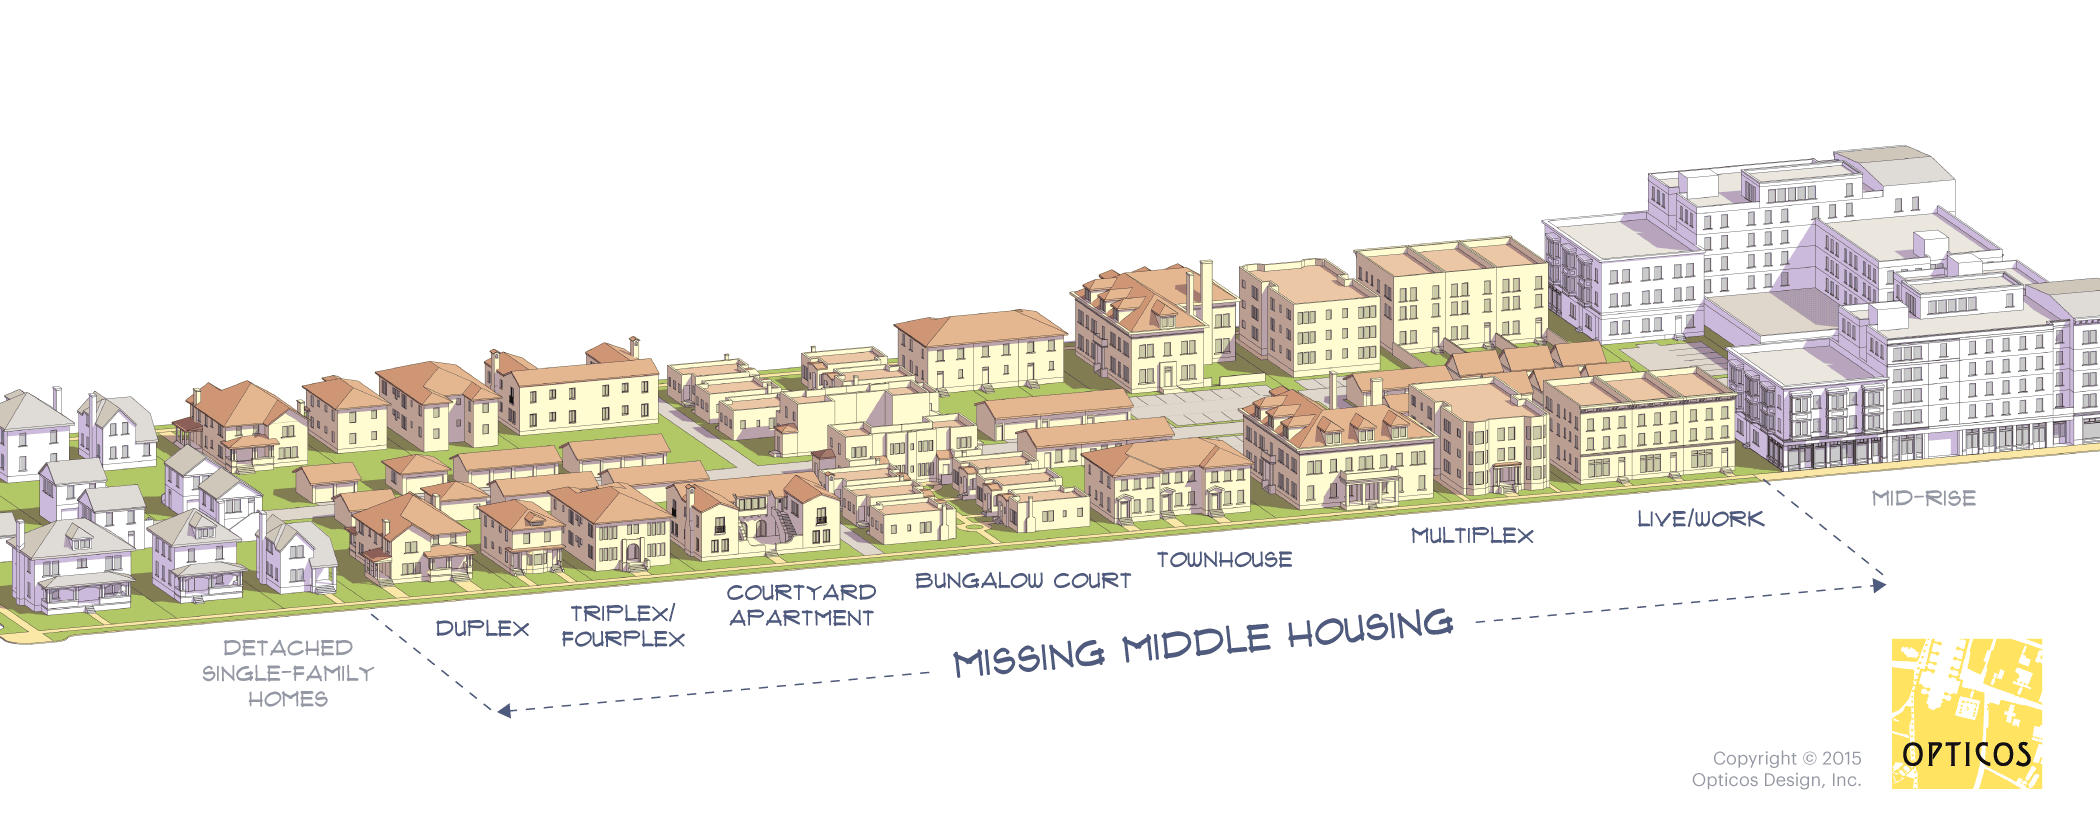
\includegraphics{assets/missing-middle.png}
\caption{Source: \href{https://missingmiddlehousing.com/}{Missing Middle Housing}}
\end{figure}

Stretching the metaphor perhaps to its breaking point, new R users at the ``detached single-family home'' stage can't get to the advanced ``mid-rise'' level without going through the middle stage. The ``missing middle'' in the R neighborhood is the lack of resources to that answer the types of nuts and bolts questions that new R users often have. Things like:

\begin{itemize}
\tightlist
\item
  How should I organize my file structure when creating a new project?
\item
  Should I do data cleaning in an RMarkdown file or an R script file?
\item
  How do I find packages? How do I know if the packages I find are high quality?
\end{itemize}

This book is my attempt to provide answers to these types of questions. It will be an opinionated look at how one person (me) uses R. I'm writing it not because I think my approach is the best and that everyone should use it. I'm writing it because I believe that I can offer some ideas that can help the students I work with -- and perhaps you as well -- to go from learning R to using it in their daily practice. R has been transformative for my work and I want it to be the same for you.

\textbf{Note}

What follows is an in-progress outline of the rest of this book. It will change over the next few months as I write the book.

\hypertarget{setting-myself-up-for-success}{%
\chapter{Setting Myself up for Success}\label{setting-myself-up-for-success}}

\hypertarget{software}{%
\section{Software}\label{software}}

\hypertarget{why-i-dont-work-just-in-r}{%
\subsection{Why I Don't Work Just in R}\label{why-i-dont-work-just-in-r}}

\hypertarget{why-i-use-rstudo-not-something-like-r-commander}{%
\subsection{Why I Use RStudo, not something like R Commander}\label{why-i-use-rstudo-not-something-like-r-commander}}

\hypertarget{rstudio-options}{%
\subsection{RStudio Options}\label{rstudio-options}}

Uncheck load data on start new session

\hypertarget{code-style}{%
\section{Code Style}\label{code-style}}

\hypertarget{examples-of-other-style-guides}{%
\subsection{Examples of other style guides}\label{examples-of-other-style-guides}}

\begin{itemize}
\tightlist
\item
  \url{http://jef.works/R-style-guide/}
\item
  \url{https://style.tidyverse.org/} + \url{https://styler.r-lib.org/index.html}
\item
  \url{https://google.github.io/styleguide/Rguide.xml}
\item
  \url{https://ropensci.github.io/dev_guide/}
\item
  \url{https://csgillespie.github.io/efficientR/}
\end{itemize}

\hypertarget{my-style-preferences}{%
\subsection{My style preferences}\label{my-style-preferences}}

\begin{itemize}
\tightlist
\item
  Spaces between things
\item
  Line breaks
\item
  Put all packages at top of script
\end{itemize}

\hypertarget{working-with-files}{%
\section{Working with Files}\label{working-with-files}}

\hypertarget{directory-organization}{%
\subsection{Directory organization}\label{directory-organization}}

\hypertarget{use-datadata-raw-structure}{%
\subsubsection{Use data/data-raw structure}\label{use-datadata-raw-structure}}

\hypertarget{naming-files}{%
\subsubsection{Naming files}\label{naming-files}}

\url{https://speakerdeck.com/jennybc/how-to-name-files?slide=3})

\hypertarget{packages}{%
\section{Packages}\label{packages}}

\hypertarget{where-do-i-find-packages}{%
\subsection{Where do I find packages?}\label{where-do-i-find-packages}}

\hypertarget{how-do-i-evaluate-packages}{%
\subsection{How do I evaluate packages?}\label{how-do-i-evaluate-packages}}

\hypertarget{why-i-use-the-tidyverse}{%
\subsection{Why I Use the Tidyverse}\label{why-i-use-the-tidyverse}}

\begin{itemize}
\tightlist
\item
  \url{https://joss.theoj.org/papers/10.21105/joss.01686}
\end{itemize}

\hypertarget{workflow}{%
\section{Workflow}\label{workflow}}

\hypertarget{when-to-use-.r-vs-.rmd}{%
\subsection{When to use .R vs .Rmd}\label{when-to-use-.r-vs-.rmd}}

Break up data cleaning (R script) and reporting (RMarkdown)

\hypertarget{load-all-data-at-top}{%
\subsection{Load all data at top}\label{load-all-data-at-top}}

\hypertarget{add-sections-in-r-scripts-to-enable-toc}{%
\subsection{Add sections in R scripts to enable TOC}\label{add-sections-in-r-scripts-to-enable-toc}}

\hypertarget{gitgithub}{%
\section{Git/GitHub}\label{gitgithub}}

Pluses

\begin{itemize}
\tightlist
\item
  Hard to get set up
\end{itemize}

Minuses

\begin{itemize}
\tightlist
\item
  Multiple people can work at a time
\item
  Version control
\item
  Branching
\end{itemize}

\hypertarget{as-compared-to-google-drive-dropbox-etc.}{%
\subsection{As compared to Google Drive, Dropbox, etc.}\label{as-compared-to-google-drive-dropbox-etc.}}

Pluses

\begin{itemize}
\tightlist
\item
  Easy
\end{itemize}

Minuses

\begin{itemize}
\tightlist
\item
  Only one person can work at a time
\item
  No version control
\end{itemize}

\hypertarget{working-with-data}{%
\chapter{Working with Data}\label{working-with-data}}

\hypertarget{importing-data}{%
\section{Importing Data}\label{importing-data}}

\hypertarget{why-to-use-read_csv-not-read.csv}{%
\subsection{Why to use read\_csv not read.csv}\label{why-to-use-read_csv-not-read.csv}}

\hypertarget{clean_names-function}{%
\subsection{clean\_names() function}\label{clean_names-function}}

\hypertarget{variable-and-value-labels}{%
\subsection{Variable and value labels}\label{variable-and-value-labels}}

\hypertarget{codebooks}{%
\subsubsection{Codebooks}\label{codebooks}}

\url{https://rubenarslan.github.io/codebook/}
\url{https://cran.r-project.org/web/packages/vtable/index.html}
\url{https://cran.r-project.org/web/packages/sjlabelled/index.html}

Include discussion of R vs SPSS

\url{http://josiahparry.com/post/2019-12-14-spss-haven/}

\hypertarget{examining-data}{%
\subsection{Examining Data}\label{examining-data}}

\begin{itemize}
\tightlist
\item
  Skimr
\item
  Naniar
\item
  DataMaid
\end{itemize}

\hypertarget{data-wrangling-and-analysis}{%
\section{Data Wrangling and Analysis}\label{data-wrangling-and-analysis}}

\hypertarget{general-practices}{%
\section{General Practices}\label{general-practices}}

\begin{itemize}
\tightlist
\item
  Restart session often\\
\item
  Create as few objects as possible\\
\item
  Load all data at top of code
\end{itemize}

\hypertarget{reporting-results-with-rmarkdown}{%
\chapter{Reporting Results with RMarkdown}\label{reporting-results-with-rmarkdown}}

Explain how I didn't use RMarkdown for a long time and really missed out

\hypertarget{general-practices-1}{%
\section{General Practices}\label{general-practices-1}}

\hypertarget{naming-code-chunks}{%
\subsection{Naming Code Chunks}\label{naming-code-chunks}}

\hypertarget{use-toc}{%
\subsection{Use TOC}\label{use-toc}}

\hypertarget{yaml}{%
\subsection{YAML}\label{yaml}}

\begin{itemize}
\tightlist
\item
  \url{https://github.com/r-lib/ymlthis}
\end{itemize}

\hypertarget{parameterized-reports}{%
\subsection{Parameterized reports}\label{parameterized-reports}}

\hypertarget{misc}{%
\subsection{Misc}\label{misc}}

\begin{itemize}
\tightlist
\item
  \url{https://github.com/ThinkR-open/remedy}
\end{itemize}

\hypertarget{tables}{%
\subsection{Tables}\label{tables}}

\hypertarget{what-format-i-knit-to-when}{%
\section{What Format I Knit To When}\label{what-format-i-knit-to-when}}

\hypertarget{word}{%
\subsection{Word}\label{word}}

Using Word reference documents for style

\hypertarget{pdf}{%
\subsection{PDF}\label{pdf}}

I basically don't because I'm scared off by LaTeX

\hypertarget{html}{%
\subsection{HTML}\label{html}}

\hypertarget{distill}{%
\subsubsection{Distill}\label{distill}}

\hypertarget{bookdown}{%
\subsubsection{Bookdown}\label{bookdown}}

\url{https://alison.rbind.io/talk/2019-rsc-bookdown/}

\hypertarget{pagedown}{%
\subsubsection{Pagedown}\label{pagedown}}

\hypertarget{dashboards}{%
\subsubsection{Dashboards}\label{dashboards}}

\hypertarget{flexdashboard}{%
\subsubsection{Flexdashboard}\label{flexdashboard}}

\hypertarget{crosstalk}{%
\paragraph{crosstalk}\label{crosstalk}}

\hypertarget{shiny}{%
\paragraph{Shiny}\label{shiny}}

\hypertarget{visualizing-data}{%
\chapter{Visualizing Data}\label{visualizing-data}}

\hypertarget{themes}{%
\section{Themes}\label{themes}}

\hypertarget{using-fonts-in-plots}{%
\section{Using Fonts in Plots}\label{using-fonts-in-plots}}

extrafont package

\hypertarget{ggplot-extensions}{%
\section{ggplot extensions}\label{ggplot-extensions}}

\hypertarget{formatting-numbers-etc}{%
\section{Formatting numbers etc}\label{formatting-numbers-etc}}

\begin{itemize}
\tightlist
\item
  Twitter tip to not use scientific notation: \url{https://twitter.com/ecologyofgavin/status/1188865515059585025}
\item
  scales package
\end{itemize}

\hypertarget{mapping}{%
\section{Mapping}\label{mapping}}

\hypertarget{general-packages}{%
\subsection{General packages}\label{general-packages}}

\begin{itemize}
\tightlist
\item
  tmap
\item
  leaflet
\item
  ggplot
\item
  mapview
\end{itemize}

\hypertarget{geocoding}{%
\subsection{Geocoding}\label{geocoding}}

\begin{itemize}
\tightlist
\item
  ggmap
\item
  \url{https://rdrr.io/cran/tmaptools/man/geocode_OSM.html}
\item
  opencage
\end{itemize}

\hypertarget{tables-1}{%
\subsection{Tables}\label{tables-1}}

See blog post

\hypertarget{what-i-do-when-things-go-wrong-and-they-always-do}{%
\chapter{What I Do When Things Go Wrong (and They Always Do)}\label{what-i-do-when-things-go-wrong-and-they-always-do}}

\hypertarget{guides-to-getting-help-in-r}{%
\section{Guides to getting help in R}\label{guides-to-getting-help-in-r}}

\begin{itemize}
\tightlist
\item
  \url{https://socviz.co/appendix.html\#a-little-more-about-r}
\item
  \url{https://sctyner.github.io/rhelp.html}
\end{itemize}

\hypertarget{read-more}{%
\chapter{Read More}\label{read-more}}

\begin{itemize}
\tightlist
\item
  \url{https://whattheyforgot.org/}
\end{itemize}

\bibliography{book.bib,packages.bib}

\end{document}
